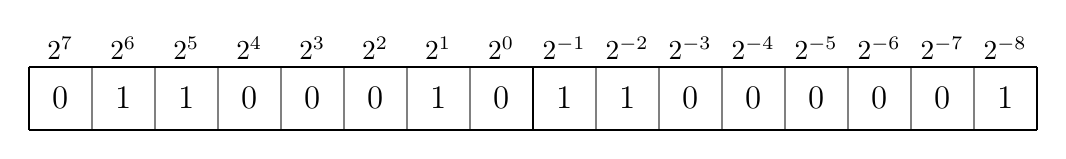
\begin{tikzpicture}[scale=0.8, every node/.style={scale=0.99}]


\colorlet{LighterMark}{black!50}

\foreach \i in {1,...,15}
{
     \draw[thick,LighterMark] (\i,1) -- (\i,0);
}

     \draw[thick,black] (0,1) -- (0,0);
      \draw[thick,black] (8,1) -- (8,0);
      \draw[thick,black] (16,1) -- (16,0);
      
\draw[thick,black] (0,0) -- (16,0);
\draw[thick,black] (0,1) -- (16,1);
 

%\foreach \i[evaluate={\pow=int(7-\i)}] in {0,...,7}
\foreach \i[evaluate={\pow=int(7-\i)}] in {0,...,7}
{
   \node[] at (\i+0.5,1.3){$2^{\pow}$  }  ;
      
         
     
}

%\foreach \i[evaluate={\pow=int((\i-7)*2)}]  in {8,...,15}
\foreach \i[evaluate={\pow=int(\i-7)}]  in {8,...,15}
{
     \node[] at (\i+0.5,1.3){$2^{-\pow}$}  ;
}

\tikzstyle{fontbf} = [font=\large]
\node[fontbf] at (0.5,0.5){0} ;
\node[fontbf] at (1.5,0.5){1};  
\node[fontbf] at (2.5,0.5){1} ; 
\node[fontbf] at (3.5,0.5){0} ;

\node[fontbf] at (4.5,0.5){0} ;
\node[fontbf] at (5.5,0.5){0};  
\node[fontbf] at (6.5,0.5){1} ; 
\node[fontbf] at (7.5,0.5){0} ;

\node[fontbf] at (8.5,0.5){1} ;
\node[fontbf] at (9.5,0.5){1};  
\node[fontbf] at (10.5,0.5){0} ; 
\node[fontbf] at (11.5,0.5){0} ;

\node[fontbf] at (12.5,0.5){0} ;
\node[fontbf] at (13.5,0.5){0};  
\node[fontbf] at (14.5,0.5){0} ; 
\node[fontbf] at (15.5,0.5){1} ;


\end{tikzpicture}
